\section{Method}
\label{sec:method}
Consider a dataset $\mathcal{D} = \{S_i\}_{i=1}^{n}$ containing $n$ sets of
shape handles.
Each set of handles $S_i$ represents a 3D shape and consists of multiple handle descriptors.
Our goal is to train a model $f_\theta$ capable of generating sets similar to the ones in
$\mathcal{D}$, i.e., using them as supervision.
More precisely, given an input $x_i$ associated with a set of handles $S_i$, our goal is to
estimate the parameters $\theta$ such that $f_\theta(x_i) \approx S_i$.
The input $x_i$ can be an image, a point cloud, an occupancy grid, or even the set of
handles itself.
When $x_i=S_i$, $f_\theta$ corresponds to an autoencoder.
If we add a regularization term to the bottleneck of $f_\theta$,
we have a Variational Auto-Encoder (VAE), which we use for
applications like shape editing, completion and interpolation (Section~\ref{sec:applications}).
However, we need to use a loss function capable of measuring the
similarity between two sets of handles, \ie the reconstruction component of a VAE.
Ideally, this loss function would be versatile -- we should be able to use it
to generate different types of handles with minimal modifications.
Moreover, our model needs to be capable of generating sets with different cardinalities,
since the sets $S_i$ do not always have the same size -- in practice,
the size of the sets used as supervision can vary a lot and our network must accommodate this need.

In this section, we describe how to create a model satisfying these constraints.
First, we describe how to compute similarities between handles.
Our method is flexible and only relies on the ability to efficiently compute the
distance from an arbitrary point in space to the handle's surface.
We then demonstrate how to use this framework with two types of handles:
cuboids and sphere-meshes.
Finally, we describe how to build models capable of generating sets with varying sizes, 
by employing a separate network branch to predict the existence of shape handles.

%The main component of our approach is a deep neural network capable of generating shapes
%represented as sets of handles.
%Our approach is versatile and can be applied to any types of handle as long as we
%are able to efficiently compute a distance from the handle to an arbitrary points in space.
%Then, we use this capability to extend well-known permutation invariant losses and
%train models capable of generating sets of handles.
%Finally, we show how to accurately generate sets with varying cardinality, creating
%a single model capable of generating shapes with a highly variable level of complexity.
%We validate our method using two representations: cuboids from the PartNet~\cite{} dataset
%and sphere-meshes computed from ShapeNet~\cite{} shapes.

\subsection{Similarity between shape handles}
\label{sec:similarity}

Consider two sets of shape handles of the same type: $A=\{a_j\}_{j=1}^{|A|}$ and $B=\{b_k\}_{k=1}^{|B|}$, where
$a_j$ and $b_k$ are parameters that describe each handle.
For example, if the handle type is cuboid, $a_j$ (or $b_k$) would include the cuboid dimensions,
rotation and translation in space.  %\rui{can a and b be different types of handles?}
One way to compute similarity between sets is through Chamfer distance.
Let the asymmetric Chamfer distance between the two sets of
handles $A$ and $B$ be defined as:
\begin{equation}
    \label{eq:ch}
    Ch(A, B) = \frac{1}{|A|}\sum_{a \in A} \min_{b \in B} D(a, b)
\end{equation}
where $D(a,b)$ is a function that computes the similarity between two handles with
parameters $a$ and $b$.
There are multiple choices for $D(a,b)$.
One straightforward choice is to define $D$ as the $\ell_p$-norm of the vector $a-b$.
However, this is a poor choice as the parameters are not homogeneous. For example, parameters that describe rotations should
not contribute to the similarity metric in the same way as those describing translations.
Furthermore, there may be multiple configurations that describe the same shape -- 
e.g., vertices that are in different orders may describe the same triangle; a cube can be rotated and translated
in multiple ways and end up occupying the same region in space.

We address these problems by proposing a novel distance metric $D(a,b)$ which measures the similarity of the distance field functions of the two handles.
Specifically, let $\mathcal{P}$ be a set of points in the 3D space and let $\mu({a})$ represent the surface of the handle described by $a$.
Now, we define $D$ as follows:
\begin{equation}
    \label{eq:D}
    D(a,b) = \sum_{p \in \mathcal{P}} \Big(\min_{p_a \in \mu(a)}\norm{p-p_a}_2 - \min_{p_b \in \mu(b)}\norm{p-p_b}_2\Big)^2
\end{equation}
Intuitively, %\rui{we should give a one-sentence descriptoin, such as essentially D calculates the L2 between the two distance field fucntions?} 
$D$ calculates the sum of squared differences between two
feature vectors representing the distance fields with respect to each of the handles.
Each dimension of these feature vectors contains the distance between a point in
a set of \emph{probe points} $\mathcal{P}$ and the surface of the handle 
defined by its parameters ($a$ and $b$ in Equation~\ref{eq:D}).
The main advantage of this similarity computation is its versatility:
it allows us to compare any types of shape handles; the only requirement
is the ability to efficiently compute $\min_{p_h \in \mu(h)}\norm{p-p_h}_2$ given
handle parameters $h$ and a point $p$.
In the following subsections, we show how to efficiently perform this computation
for two types of shape handles: cuboids and sphere-meshes.

\paragraph*{Cuboids.}
We choose to represent a cuboid by parameters
$h = \langle\bf c, \bf l , \bf r_1, \bf r_2\rangle$, where $\mathbf{c} \in \mathbb{R}^3$ is the cuboid center, $\mathbf{l} \in \mathbb{R}^3$ is the cuboid scale factor (i.e. dimensions), $\mathbf{r_1}, \mathbf{r_2} \in \mathbb{R}^3$ are vectors describing the
rotation of the cuboid.
This rotation representation has continuity properties that benefit
its estimation through neural networks~\cite{nnrotation}.
Notice that we can build a rotation matrix $\bf R$ from $\bf r_1$ and $\bf r_2$
by following the procedure described in~\cite{nnrotation}.
Now, consider the transformation $\tau_h(p) = \mathbf{R}^Tp - \mathbf{c}$.
Let $\mu_C(h) \in \mathbb{R}^3$ represent the surface of the cuboid parametrized by $h$. We can compute $\min_{p_h \in \mu_C(h)}\norm{p-p_h}_2$
(i.e. distance from $p$ to the cuboid) as follows: %\duygu{shouldn't we have \bf{l/2} instead of \bf{l}}
$$
\min_{p_h \in \mu_C(h)}\norm{p-p_h}_2 = 
\norm{(|\tau_h(p)| - \bf l)^+}_2 + \big(\max(|\tau_h(p)| - \mathbf{l})\big)^-
$$
where $(\cdot)^+$, $(\cdot)^-$ and $|\cdot|$ represent element-wise $\max(\cdot, 0)$, $\min(\cdot, 0)$ and absolute value, respectively.
Since this expression can be computed in $O(1)$, 
we are able to compute Equation~\ref{eq:D} in $O(|\mathcal{P}|)$, where the number of probing points $|\mathcal{P}|$ is relatively small.
In practice, we sample 64 points in a regular grid
in the unit cube.

\paragraph*{Sphere-meshes.}

\begin{figure}
\centering
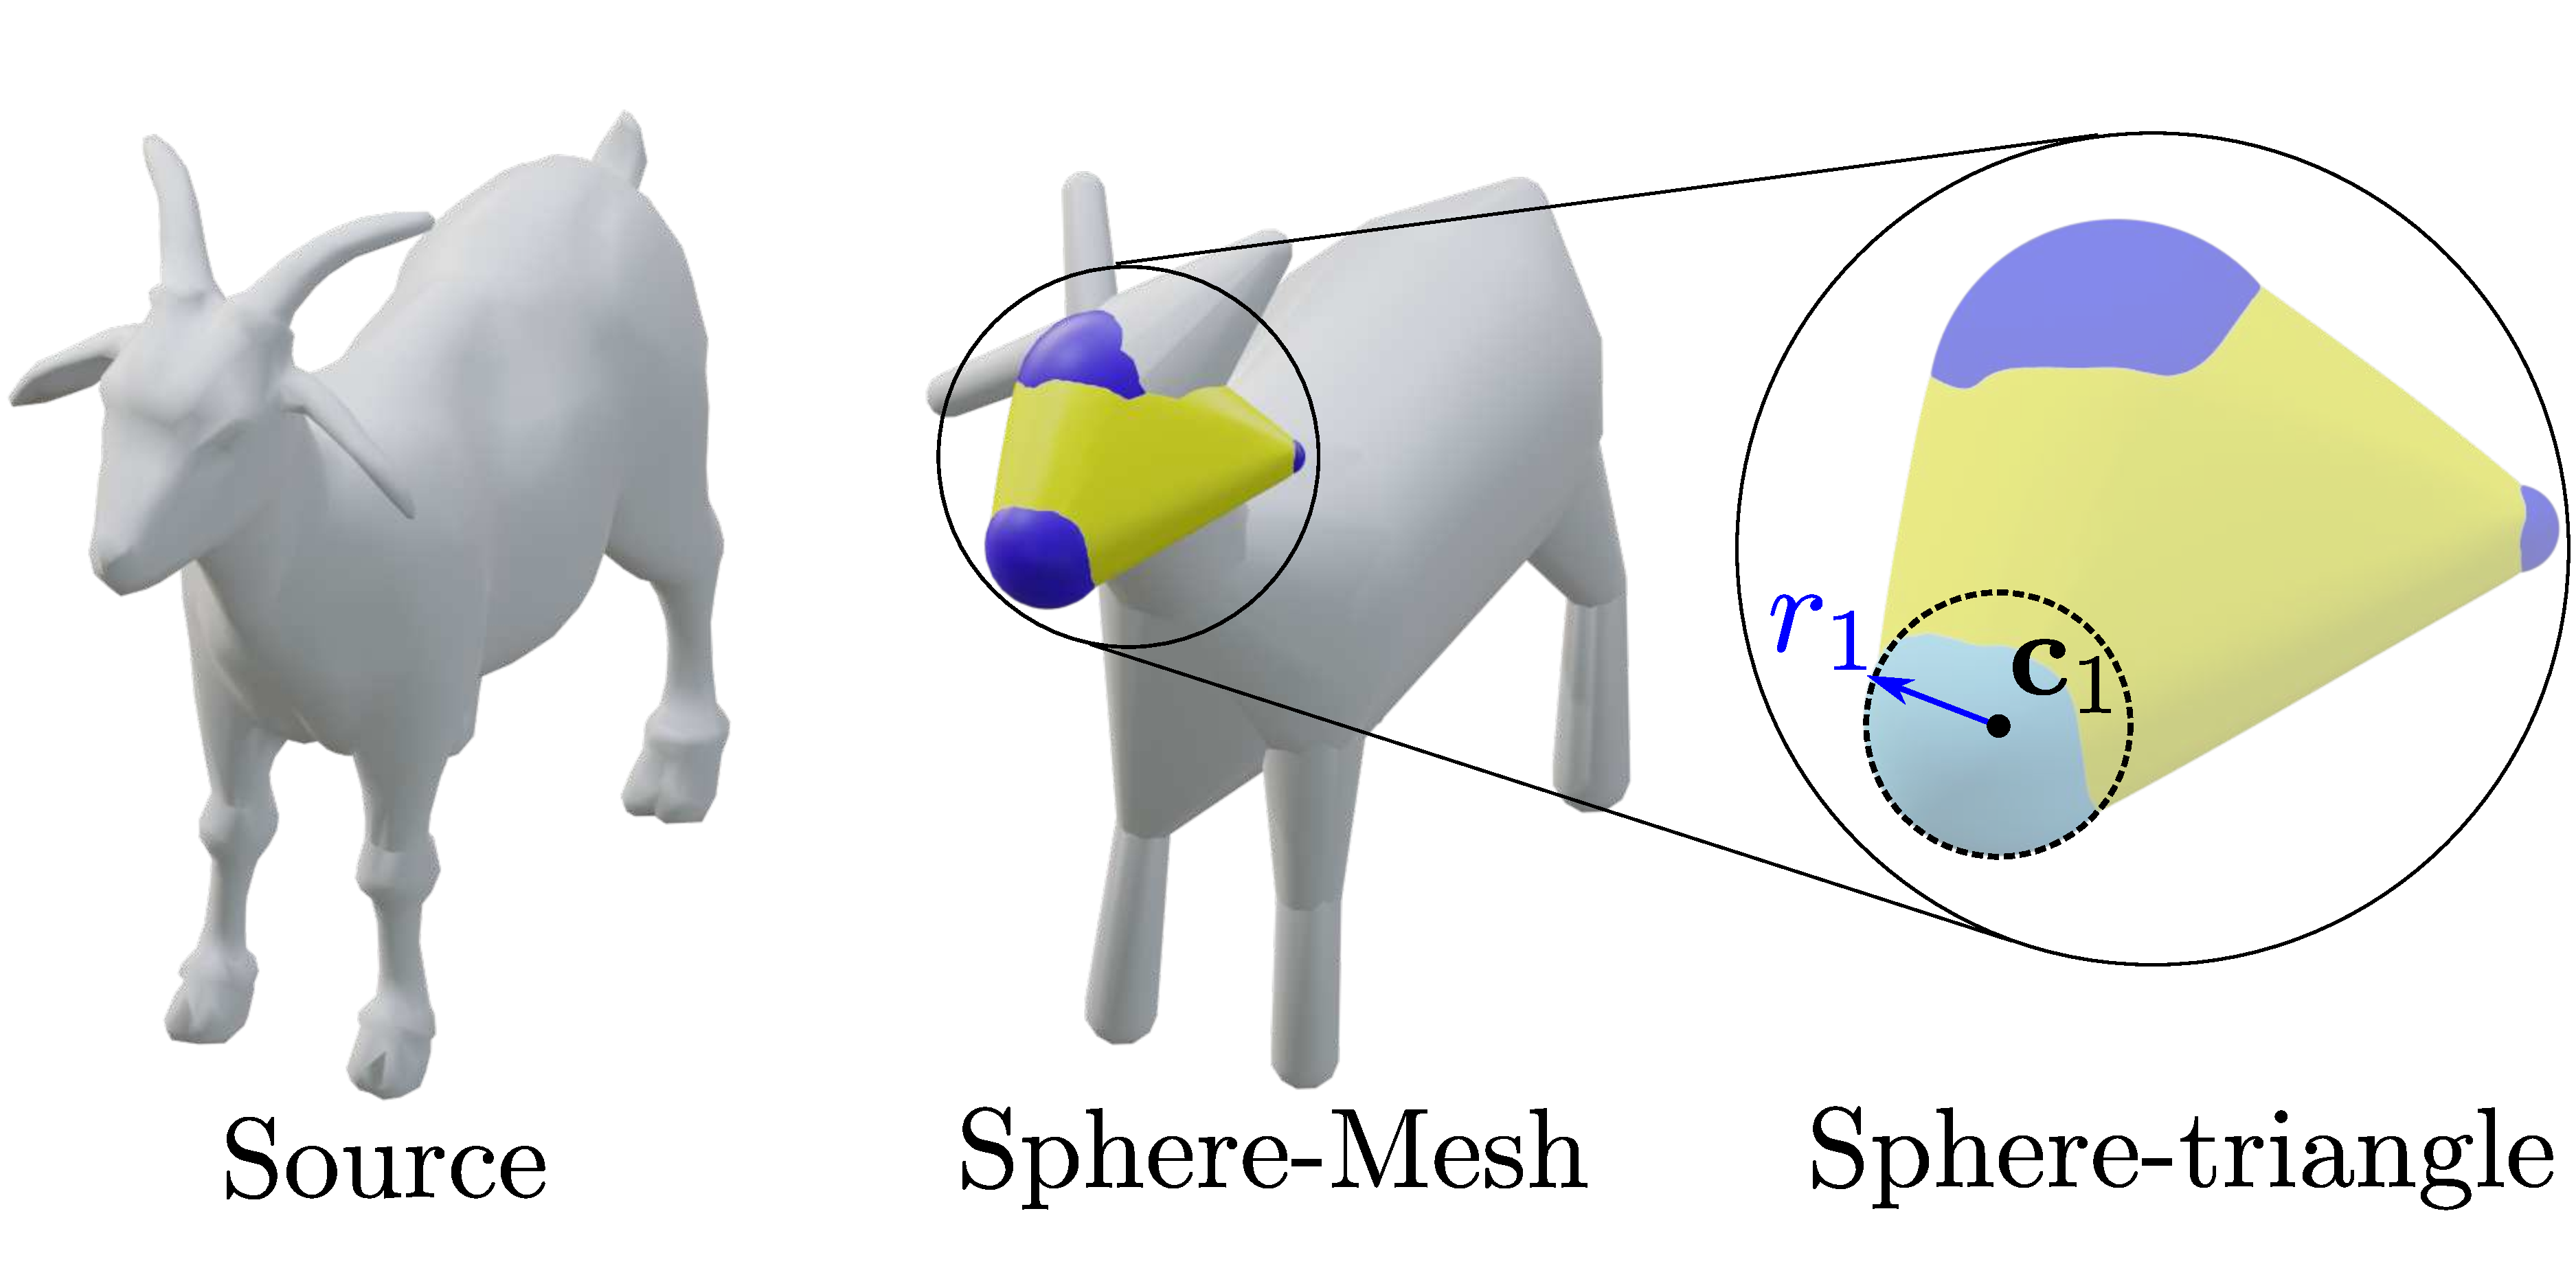
\includegraphics[width=0.8\linewidth]{handles/imgs/spheremesh_explained.pdf}
\caption{\label{fig:spheremesh} \small
Schematic representation of sphere-meshes.
A sphere-mesh (middle) is computed from a regular triangle mesh (left) as input, and it consists of multiple sphere-triangles (right), each of which is a volumetric representation}
\end{figure}

A triangle mesh consists of a set of vertices and triangular faces representing
the vertex connectivity.
Every vertex is a point in space and the surface of a triangle contains all the points
that can be generated by interpolating the triangle's vertices using
barycentric coordinates.
A sphere-mesh is a generalization of a triangle mesh -- every vertex is
a sphere instead of a point in space.
Thus, every sphere-mesh ``triangle" is actually a volume delimited by the convex-hull
of the spheres centered at the triangle vertices.
Figure~\ref{fig:spheremesh} presents a visual description of sphere-mesh components.
Thiery et al.~\cite{spheremesh} introduced an algorithm to compute sphere-meshes from
regular triangle meshes.
They show that complex meshes can be closely approximated with a sphere-mesh containing
a fraction of the original components.

We model sphere-meshes as a set of sphere-mesh triangles, called \emph{sphere-triangles}.
Similarly to a regular triangle, a sphere-triangle is fully defined by 
its vertices, the difference being that its vertices are now spheres instead of
points.
Thus, we choose to represent a sphere-triangle using parameters
$h = \langle r_1, r_2, r_3, \bf c_1, c_2, c_3 \rangle$; where 
$\mathbf{c_1}, \mathbf{c_2}, \mathbf{c_3} \in \mathbb{R}^3$
are the centers of the three spheres, and $r_1, r_2, r_3 \in \mathbb{R}^+$ are
their radii.
Let $\mu_T(h)$ represent the the surface of the sphere-triangle parametrized by $h$.
For calculating the similarity between two sphere-triangles: as each sphere-triangle is uniquely defined by its three spheres, it suffices to have $\mu_T$ contain only the surfaces of these three spheres, and hence it does not need to contain the entire sphere triangle.
Thus, the distance of a probing point $p$ to the handle surface is computed as follows:
$$
\min_{p_h \in \mu_T(h)}\norm{p-p_h}_2 = 
\min_{i\in\{1, 2, 3\}} (\norm{p - \mathbf{c}_i}_2 - r_i).
$$

\subsection{Generating sets with varying cardinality}
\label{sec:cardinality}
%\duygu{Here shall we also say in 1-2 sentences that it is easier to set a maximum fixed number of handles to predict and thus we need to additionally predict whether each handle actually exists or not}
The neural network $f$ generates shapes represented by sets of handles given an input $x$.
Our design of $f$ includes two main components: an encoder $q$ that, given an input $x$, outputs a latent set representation
$z$; and a decoder $g$ that, given the latent set representation $z$, generates
a set of handles.
Even though we can use a symmetric version of Equation~\ref{eq:ch} 
to compute the similarity between the generated set $g(q(x_i))$ 
and the ground-truth set of handles $S_i$, 
so far our model has not taken into account the varying size (i.e. number of elements) of the generated sets.
We address this issue by separating the generator into two parts: a parameter prediction
branch $g_p$ and an existence prediction branch $g_e$. The parameter prediction branch is trained to always output a fixed number of handle parameters where
$[g_p(z)]_i$ represents the parameters of the $i^{th}$ handle. On the other hand, the existence prediction branch $[g_e(z)]_i \in [0,1]$ represents the probability of existence of the $i^{th}$
generated handle.
Now, we need to adapt our loss function to consider the probability of
existence of a handle.

If we assume that all handles exist, our model can be trained using the following
loss: %\duygu{shall we call this $\mathcal{L}_{rec}$ since it is referred as the reconstruction loss later}
$$
\mathcal{L} = Ch(g_p(z_i), S_i) + Ch(S_i, g_p(z_i)),
$$
where $S_i$ is a set of shape handles drawn from the training data and
$z_i$ is a latent representation computed from the associated input $x_i$.
However, we want to modify this loss to take into account the probability of a handle existing
or not. To do so, note that $\mathcal{L}$ has two terms.
The first term measures accuracy: i.e. how close each of the handles in $g_p(z_i)$ is from the handles
in $S_i$.
For this term, we can use $g_e$ as weights for the summation in Equation~\ref{eq:ch},
which leads to the following definition:
\begin{equation}
\label{eq:prec}
P(z, S) = \sum_{i=1}^K \min_{s \in S} D([g_p(z)]_i, s)[g_e(z)]_i,
\end{equation}
where $z$ is a latent space representation,  $S$ is a set of handles and
$K = |g_p(z)| = |g_e(z)|$.
The intuition is quite simple:
if the $i^{th}$ handle is likely to exist, its distance to the closest handle should be taken into consideration;
on the other hand, if the $i^{th}$ handle is unlikely to exist, it does not matter if
it is approximating a handle in $S$ or not.

The second term in $\mathcal{L}$ measures coverage:
every handle in $S_i$ must have (at least) one handle in the generated set that is very
similar to it.
Here, we use an insight presented in~\cite{Paschalidou2019} to efficiently compute the coverage of
$S_i$ while considering the probability of elements in a set existing or not.
Let $g_p^s(z)$ be the list of generated handles $g_p(z)$ ordered in non-decreasing
order according to $D([g_p^s]_i, s)$ for $i=1,...,|g_p(z)|$.
We compute the coverage of a set $S$ from a set generated from $z$ as follows:
\begin{equation}
    \label{eq:cov}
C(z, S) = \sum_{s \in |S|} \sum_{i=1}^{K}D([g_p^s(z)]_i, s)[g_e^s(z)]_i \prod_{j=1}^{i-1}(1 - [g_e^s(z)]_j).
\end{equation}
The idea behind this computation is the following:
for every handle $s \in S$, we compute its distance to every handle in $g_p(z)$, weighted
by the probability of that handle existing or not.
However, the distance to a specific handle is important only if no other handle closer to $s$ exists. Thus, the whole term needs to be weighted by $\prod_{j=1}^{i}(1 - [g_e^s(z)]_j)$.
Finally, we can combine Equations~\ref{eq:prec} and \ref{eq:cov} to define the
reconstruction loss $\mathcal{L}_{rec}$ used to train our model:
\begin{equation}
    \label{eq:rec}
    \mathcal{L}_{rec} = P(z, S) + C(z, S).
\end{equation}

\paragraph{Alternate training procedure.}
\begin{figure}
\centering
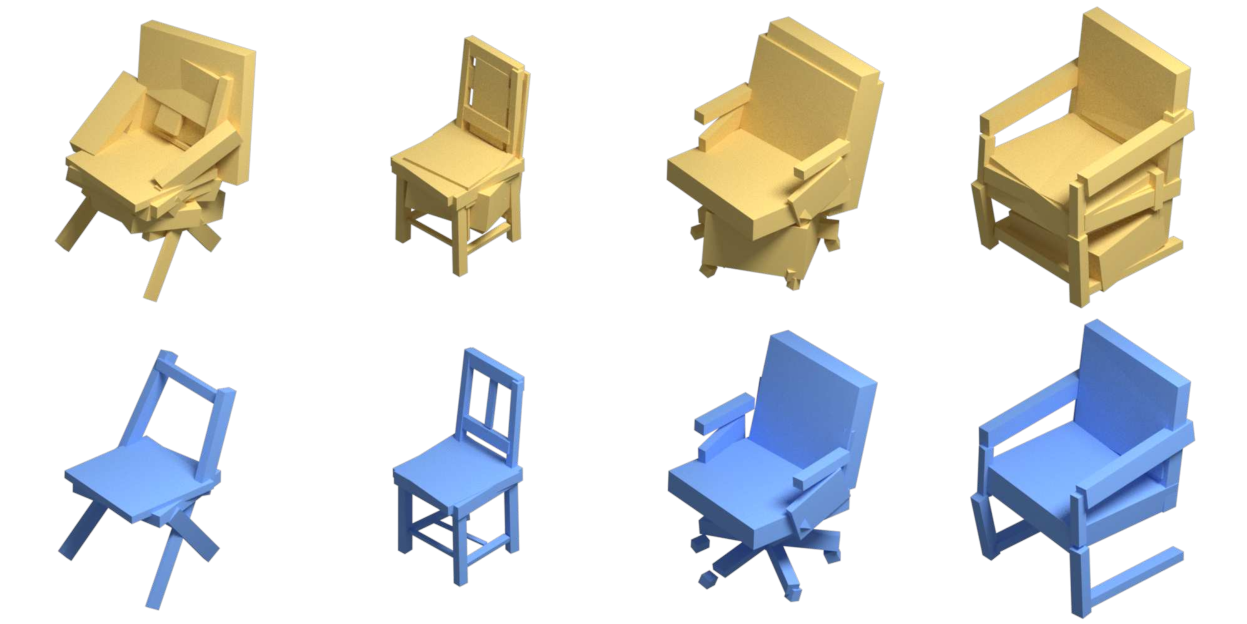
\includegraphics[width=0.8\linewidth]{handles/imgs/stagecomp.pdf}
\caption{\label{fig:alttrain} \small
Comparison of results after the first stage (top row) and second
stage (bottom row) of alternate training.
While the first stage ensures coverage, some extra, unnecessary handles are also generated.
The second stage trains the existence branch, which assigns a low probability
of existence to the inaccurate handles.}
\end{figure}

Although minimizing the loss in Equation~$\ref{eq:rec}$ at once enables
generating sets of different sizes, our experiments show that the
results can be further improved if we train $g_p$ and $g_e$ in an alternating fashion.
Specifically, we first initialize the biases and weights of the last layer of $g_e$ to ensure
that all of its outputs are $1$, i.e., the model is initialized to predict that every primitive exists.
Then, in the first stage of the training, we fix the parameters of $g_e$ and train $g_p$ minimizing only the coverage
$C(z, S)$.
During the second stage of the training, we fix the parameters of $g_p$ and
update the parameters of $g_e$, but this time minimizing the full reconstruction loss
$\mathcal{L}_{rec}$.
As we show in Section 4, this alternating procedure improves the training leading to the generation of more
accurate shape handles.  
The intuition is that while training the model to predict the handle parameters ($g_p$), the
network should be only concerned about coverage, i.e., generating at least one similar handle for each 
ground-truth handle.
On the other hand, while training the existence prediction branch ($g_e$), we want
to remove the handles that are in incorrect positions while keeping the coverage of the ground-truth set. %\duygu{the existence prediction removes the redundant handles, no? isn't the first branch responsible for removing the incorrect handles}

